\documentclass[11pt]{article}
\usepackage{amsmath, amssymb, physics, mathtools, bm}
\usepackage{tikz, pgfplots}
\usetikzlibrary{decorations.pathmorphing, decorations.markings, arrows.meta, calc}
\pgfplotsset{compat=1.18}
\usepackage[margin=2.3cm]{geometry}
\usepackage{siunitx, booktabs, hyperref}
\usepackage{braket}

\newcommand{\D}{\mathrm{D}}
\newcommand{\de}{\mathrm{d}}
\newcommand{\pd}[2]{\frac{\partial #1}{\partial #2}}
\newcommand{\pdd}[2]{\frac{\partial^{2} #1}{\partial #2^{2}}}
\newcommand{\Lap}{\nabla^{2}}

\title{B4 Nuclear and Particle Physics, 2021 --- Model Solutions}
\author{}
\date{}

\begin{document}
\maketitle

%==========================================================
\section*{Question 1 --- Conservation laws, $e^{+}e^{-}$ collisions and the $Z^{0}$}

\textbf{Problem.} Discuss colour and flavour conservation; explain $e^{+}e^{-}\to\mu^{+}e^{-}+\text{missing}$; find the two-EM-shower fraction of $\tau\tau$ at a $\mu^{+}\mu^{-}$ collider; ratio of $e^{+}e^{-}$ to hadronic interactions just below the $Z^{0}$ peak.

\subsection*{(a) Colour and flavour conservation}

\emph{Colour.} $\mathrm{SU(3)_{C}}$ exact gauge symmetry: every QCD vertex conserves colour; $\gamma$, $W^{\pm}$, $Z^{0}$ are colour singlets, so EM and weak vertices also conserve colour. Evidence: $R\equiv\sigma(e^{+}e^{-}\to\text{had})/\sigma(e^{+}e^{-}\to\mu^{+}\mu^{-})=N_{c}\sum_{q}e_{q}^{2}$ requires $N_{c}=3$; $\Gamma(\pi^{0}\to\gamma\gamma)\propto N_{c}^{2}$; three jets in $e^{+}e^{-}\to q\bar q g$.

\emph{Quark flavour.} Strong + EM diagonal in flavour (vertices conserve $S,C,B,T,I_{3}$). Charged current $W^{\pm}$ violates flavour via CKM ($\Delta S=\pm 1$ at one vertex); neutral current $Z^{0}$ is flavour-diagonal at tree level (GIM). Evidence: $K^{0}\!\leftrightarrow\!\bar K^{0}$ oscillations, $K^{+}\to\mu^{+}\nu$, $B\to D\ell\nu$; suppression of $K_{L}\to\mu^{+}\mu^{-}$ confirms GIM.

\emph{Lepton flavour.} $L_{e},L_{\mu},L_{\tau}$ each conserved at all vertices in the SM (massless-$\nu$ limit); broken only by neutrino oscillation in propagation. Evidence: $\mathrm{BR}(\mu\to e\gamma)<10^{-13}$; success of $\mu^{-}\to e^{-}\bar\nu_{e}\nu_{\mu}$.

\subsection*{(b) Two SM channels for $e^{+}e^{-}\to\mu^{+}e^{-}+\text{missing}$}

Visible $L_{e}=+1$, $L_{\mu}=-1$, $Q=0$: missing must carry $L_{e}=-1$, $L_{\mu}=+1$.

\emph{Channel 1: $W$-pair production}, $\sqrt{s}\gtrsim 2M_{W}\simeq 161\,\text{GeV}$:
\[
e^{+}e^{-}\to Z^{0}/\gamma^{*}\to W^{+}W^{-},\qquad W^{+}\to\mu^{+}\nu_{\mu},\;W^{-}\to e^{-}\bar\nu_{e}.
\]
Branching $\mathrm{BR}(W\to\ell\nu)\simeq 1/9$ per flavour; rate $\propto(1/9)^{2}$ of $\sigma_{WW}$.

\emph{Channel 2: $\tau$-pair production}, $\sqrt{s}\geq 2m_{\tau}\simeq 3.5\,\text{GeV}$ (rate maximised at the $Z^{0}$ pole):
\[
e^{+}e^{-}\to\gamma^{*}/Z^{0}\to\tau^{+}\tau^{-},\qquad\tau^{+}\to\mu^{+}\nu_{\mu}\bar\nu_{\tau},\;\tau^{-}\to e^{-}\bar\nu_{e}\nu_{\tau}.
\]

\textbf{Feynman diagram (Channel 1).} \emph{$e^{+}e^{-}$ annihilate at a vertex into $s$-channel $\gamma^{*}/Z^{0}$ which couples to $W^{+}W^{-}$ at a second vertex; $W^{+}\to\mu^{+}\nu_{\mu}$ and $W^{-}\to e^{-}\bar\nu_{e}$ at the two leptonic vertices.}

\textbf{Feynman diagram (Channel 2).} \emph{$e^{+}e^{-}$ annihilate via $s$-channel $\gamma^{*}/Z^{0}$ into $\tau^{+}\tau^{-}$; each $\tau$ decays via its own $W$ propagator: $\tau^{+}\to\bar\nu_{\tau}W^{+}$, $W^{+}\to\mu^{+}\nu_{\mu}$; $\tau^{-}\to\nu_{\tau}W^{-}$, $W^{-}\to e^{-}\bar\nu_{e}$.}

\textbf{Missing-energy sketches.}

Channel 1: each $W$ decay is two-body, $E_{\ell}^{*}=M_{W}/2$ in the $W$ rest frame (isotropic). Boost to lab ($E_{W}=\sqrt{s}/2$, $p_{W}=\sqrt{s/4-M_{W}^{2}}$) flattens the spectrum:
\[
E_{\ell}^{\text{lab}}\in\bigl[\tfrac12(E_{W}-p_{W}),\,\tfrac12(E_{W}+p_{W})\bigr].
\]
Two flat (box) charged-lepton spectra convolve to a triangular missing-energy distribution centred at $\sqrt{s}/2$.

Channel 2: leptonic $\tau$ decay has the Michel spectrum, charged-lepton energy
\[
\frac{1}{\Gamma}\frac{\de\Gamma}{\de x}=2x^{2}(3-2x),\qquad x=2E_{\ell}/m_{\tau},
\]
peaked at $x=1$. Boosting to lab gives a softer charged-lepton spectrum, hence a missing-energy distribution that is broad and unimodal, peaking near $\sim 0.7\sqrt{s}$.

\begin{center}
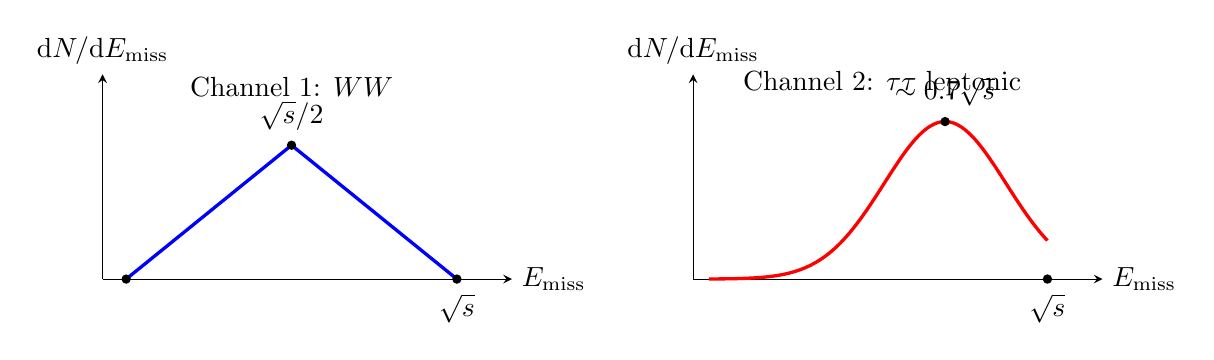
\begin{tikzpicture}[>=stealth, scale=1.0]
\begin{scope}
  \draw[->] (0,0)--(5.2,0) node[right]{$E_\text{miss}$};
  \draw[->] (0,0)--(0,2.6) node[above]{$\de N/\de E_\text{miss}$};
  \draw[blue, very thick] (0.3,0)--(2.4,1.7)--(4.5,0);
  \node[circle,fill,inner sep=1.2pt,label={above:{$\sqrt{s}/2$}}] at (2.4,1.7) {};
  \node[circle,fill,inner sep=1.2pt] at (0.3,0) {};
  \node[circle,fill,inner sep=1.2pt,label=below:{$\sqrt{s}$}] at (4.5,0) {};
  \node[above] at (2.4,2.2) {Channel 1: $WW$};
\end{scope}
\begin{scope}[xshift=7.5cm]
  \draw[->] (0,0)--(5.2,0) node[right]{$E_\text{miss}$};
  \draw[->] (0,0)--(0,2.6) node[above]{$\de N/\de E_\text{miss}$};
  \draw[red, very thick, smooth, samples=80, domain=0.2:4.5] plot ({\x},{2.0*exp(-pow(\x-3.2,2)/1.2)});
  \node[circle,fill,inner sep=1.2pt,label={above:{$\sim 0.7\sqrt{s}$}}] at (3.2,2.0) {};
  \node[circle,fill,inner sep=1.2pt,label=below:{$\sqrt{s}$}] at (4.5,0) {};
  \node[above] at (2.4,2.2) {Channel 2: $\tau\tau$ leptonic};
\end{scope}
\end{tikzpicture}
\end{center}

\boxed{\;e^{+}e^{-}\to W^{+}W^{-}\to(\mu^{+}\nu_{\mu})(e^{-}\bar\nu_{e}),\qquad e^{+}e^{-}\to\tau^{+}\tau^{-}\to(\mu^{+}\nu_{\mu}\bar\nu_{\tau})(e^{-}\bar\nu_{e}\nu_{\tau}).\;}

\subsection*{(c) Two-EM-shower $\tau$-pair fraction}

At $\sqrt{s}=M_{Z}$, $Z^{0}\to\tau^{+}\tau^{-}$ produces back-to-back taus. ``Two high-energy EM showers fully contained in the EMCAL'', with no muon track and no hadronic activity, requires both taus to decay leptonically to electrons:
\[
\tau\to e\,\bar\nu_{e}\nu_{\tau},\qquad\mathrm{BR}\simeq 17.8\%.
\]
Both legs:
\[
P_{ee}\;=\;[\mathrm{BR}(\tau\to e\nu\bar\nu)]^{2}\;=\;(0.178)^{2}.
\]
Evaluate:
\begin{equation}
\boxed{\;P_{ee}\simeq 3.2\%.\;}
\end{equation}

\subsection*{(d) $e^{+}e^{-}/\text{hadrons}$ a few MeV below the $Z^{0}$ peak}

On the $Z^{0}$ resonance the cross-section ratio reduces to a partial-width ratio:
\[
\frac{\sigma(e^{+}e^{-}\to e^{+}e^{-})}{\sigma(e^{+}e^{-}\to\text{had})}\;=\;\frac{\Gamma_{ee}}{\Gamma_\text{had}}.
\]
Lepton universality: $\Gamma_{ee}=\Gamma_{\mu\mu}=\Gamma_{\tau\tau}\simeq 83.9\,\text{MeV}$; PDG $\Gamma_\text{had}\simeq 1744\,\text{MeV}$. Substitute:
\[
\frac{\Gamma_{ee}}{\Gamma_\text{had}}\;=\;\frac{83.9}{1744}.
\]
Evaluate:
\begin{equation}
\boxed{\;\frac{N(e^{+}e^{-})}{N(\text{had})}\;\simeq\;4.8\%.\;}
\end{equation}
Equivalently $R_{Z}\equiv\Gamma_\text{had}/\Gamma_{\ell\ell}\simeq 20.8$, consistent with five accessible quark flavours $\times\,N_{c}=3$ weighted by electroweak couplings.

%==========================================================
\section*{Question 2 --- Bubble-chamber identification and the $\Delta(1232)$}

\textbf{Problem.} List conserved quantum numbers; identify charged tracks; deduce neutrals $X,Y$ in $\pi^{-}p$ event; mass and lifetime of the $\pi^{+}p$ resonance; non-relativistic Breit--Wigner shape and deviations.

\subsection*{(a) Conserved quantum numbers}

\begin{center}\small
\begin{tabular}{lccc l}
\toprule
Quantity & S & EM & W & Comment\\
\midrule
$E$, $\bm p$, $\bm J$ & \checkmark & \checkmark & \checkmark & spacetime symmetries\\
Charge $Q$ & \checkmark & \checkmark & \checkmark & $\mathrm{U(1)_{EM}}$\\
Colour & \checkmark & \checkmark & \checkmark & $\mathrm{SU(3)_{C}}$ exact\\
Baryon $B$ & \checkmark & \checkmark & \checkmark & accidental global $\mathrm{U(1)}$\\
Lepton family $L_{\ell}$ & \checkmark & \checkmark & \checkmark$^{*}$ & $^{*}$broken by $\nu$ oscillations\\
Quark flavour $S,C,B,T$ & \checkmark & \checkmark & $\times$ & CKM at $W$ vertex\\
$P$ & \checkmark & \checkmark & $\times$ & maximal $P$ violation in W\\
$C$ & \checkmark & \checkmark & $\times$ & \\
$CP$/$T$ & \checkmark & \checkmark & $\times$ & CKM, PMNS phases\\
Isospin $I$ & \checkmark$^{\dagger}$ & $\times$ & $\times$ & $^{\dagger}$$m_{u}\neq m_{d}$\\
$G$-parity & \checkmark$^{\dagger}$ & $\times$ & $\times$ & approximate\\
\bottomrule
\end{tabular}
\end{center}

\subsection*{(b) Identification of charged tracks}

Magnetic rigidity $p=qBR$ from track curvature gives momentum (sign $\Rightarrow$ charge sign). Calorimetric energy $E$ at terminus combined with $p$ gives $m^{2}=E^{2}-p^{2}c^{2}$, hence species. $\de E/\de x$ ionisation, time-of-flight, or Cherenkov supplement when $\beta\to 1$.

\subsection*{(c) Identification of $X$ and $Y$}

Initial state: $\pi^{-}p$ has $Q=0$, $B=+1$, $S=0$, $L_{\ell}=0$.

\emph{Vertex producing $\pi^{+}\pi^{-}$ (downstream).} Neutral parent ($B=0$) decays to $\pi^{+}\pi^{-}$. Strangeness-zero candidates ($\rho^{0}$, $\omega$, $f^{0}$) decay strongly with $c\tau\ll 1\,\text{fm}$, no visible flight. Visible vee in a chamber requires weak decay: $K^{0}_{S}\to\pi^{+}\pi^{-}$ (BR $69\%$, $c\tau=2.68\,\text{cm}$). Strangeness $|S|=1$.
\[
\boxed{\;X=K^{0}_{S}.\;}
\]

\emph{Vertex producing $p\pi^{-}$.} Neutral with $B=+1$, decaying to $p+\pi^{-}$. Candidates: $\Lambda(uds)\to p\pi^{-}$ ($c\tau=7.89\,\text{cm}$) or $\Sigma^{0}\to\Lambda\gamma$. The hint $\Sigma^{0}\to\Lambda\gamma$ is electromagnetic with $\tau\sim 7\times 10^{-20}\,\text{s}$, $c\tau\sim 2\times 10^{-11}\,\text{m}$: any $\Sigma^{0}$ decays before leaving a track, so the visible neutral track is the $\Lambda$ itself (whether produced directly or via $\Sigma^{0}\to\Lambda\gamma$).

Strangeness conservation in strong production: $X$ carries $S=+1$, so $Y$ must carry $S=-1$. Both $\Lambda$ and $\Sigma^{0}$ have $S=-1$. Visible flight pattern selects $\Lambda$ as the chamber-traversing neutral:
\[
\boxed{\;Y=\Lambda.\;}
\]

Production reaction (associated production):
\[
\pi^{-}+p\to\Lambda+K^{0}_{S},\qquad\Lambda\to p\pi^{-},\qquad K^{0}_{S}\to\pi^{+}\pi^{-}.
\]

\subsection*{(d) Mass and lifetime of the $\pi^{+}p$ resonance}

Read off graph: peak at $T_{\pi}^{\text{peak}}\simeq 195\,\text{MeV}$, FWHM $\Delta T_{\pi}\simeq 180\,\text{MeV}$.

Invariant mass squared, fixed-target ($p$ at rest):
\begin{equation}
s\;=\;m_{\pi}^{2}+m_{p}^{2}+2m_{p}E_{\pi}^{\text{lab}},\qquad E_{\pi}^{\text{lab}}=T_{\pi}+m_{\pi}.
\label{eq:s-fixed}
\end{equation}
Substitute $m_{\pi}=139.6\,\text{MeV}$, $m_{p}=938.3\,\text{MeV}$, $T_{\pi}=195\,\text{MeV}$:
\[
E_{\pi}^{\text{lab}}\;=\;195+139.6\;=\;334.6\,\text{MeV}.
\]
Insert into \eqref{eq:s-fixed}:
\[
s\;=\;(0.1396)^{2}+(0.9383)^{2}+2(0.9383)(0.3346)\,\text{GeV}^{2}.
\]
Evaluate:
\[
s\;=\;0.0195+0.8804+0.6280\;=\;1.528\,\text{GeV}^{2}.
\]
Take the square root:
\[
\sqrt{s}\;=\;1.236\,\text{GeV}.
\]
\begin{equation}
\boxed{\;M_{R}\simeq 1.23\,\text{GeV}/c^{2}\quad(\Delta(1232)).\;}
\end{equation}

Width transform: differentiate \eqref{eq:s-fixed} at fixed $m_{\pi},m_{p}$:
\[
2\sqrt{s}\,\Delta\sqrt{s}\;=\;2m_{p}\,\Delta T_{\pi}.
\]
Solve for $\Gamma\simeq\Delta\sqrt{s}$:
\[
\Gamma\;=\;\frac{m_{p}}{\sqrt{s}}\,\Delta T_{\pi}.
\]
Substitute:
\[
\Gamma\;=\;\frac{0.938}{1.236}\times 180\,\text{MeV}\;=\;137\,\text{MeV}.
\]
Lifetime $\tau=\hbar/\Gamma$:
\[
\tau\;=\;\frac{6.58\times 10^{-22}\,\text{MeV}\,\text{s}}{137\,\text{MeV}}.
\]
Evaluate:
\begin{equation}
\boxed{\;\Gamma\simeq 137\,\text{MeV},\qquad\tau\simeq 4.8\times 10^{-24}\,\text{s}.\;}
\end{equation}
Strong-decay timescale, consistent with PDG ($\Gamma=117\,\text{MeV}$).

\subsection*{(e) Non-relativistic Breit--Wigner and deviations}

Single isolated partial wave, projectile spins $s_{1}=0$ ($\pi$), $s_{2}=1/2$ ($p$), $J=3/2$ ($\Delta$):
\begin{equation}
\sigma_\text{el}(E)\;=\;\frac{4\pi}{k^{2}}\,\frac{2J+1}{(2s_{1}+1)(2s_{2}+1)}\,\frac{\Gamma^{2}/4}{(E-E_{R})^{2}+\Gamma^{2}/4}.
\label{eq:BW-NR}
\end{equation}
Spin factor:
\[
\frac{2J+1}{(2s_{1}+1)(2s_{2}+1)}\;=\;\frac{4}{1\cdot 2}\;=\;2.
\]
On peak:
\[
\sigma_\text{el}^\text{peak}\;=\;\frac{8\pi}{k_{R}^{2}}.
\]
CM wavenumber from \eqref{eq:s-fixed}:
\[
k_{R}^{2}\;=\;\frac{[s-(m_{\pi}+m_{p})^{2}][s-(m_{\pi}-m_{p})^{2}]}{4s}.
\]
Substitute $s=1.528\,\text{GeV}^{2}$, $(m_{\pi}+m_{p})^{2}=1.162$, $(m_{\pi}-m_{p})^{2}=0.638\,\text{GeV}^{2}$:
\[
k_{R}^{2}\;=\;\frac{(1.528-1.162)(1.528-0.638)}{4\times 1.528}\,\text{GeV}^{2}\;=\;\frac{0.366\times 0.890}{6.112}\,\text{GeV}^{2}.
\]
Evaluate:
\[
k_{R}^{2}\;=\;0.0533\,\text{GeV}^{2}\;\Rightarrow\;k_{R}\simeq 231\,\text{MeV}.
\]
Peak cross-section using $1\,\text{GeV}^{-2}=0.389\,\text{mb}$:
\[
\sigma_\text{el}^\text{peak}\;=\;\frac{8\pi}{0.0533}\,\text{GeV}^{-2}\;=\;471\,\text{GeV}^{-2}\;=\;471\times 0.389\,\text{mb}.
\]
\begin{equation}
\boxed{\;\sigma_\text{el}^\text{peak}\simeq 184\,\text{mb},\;}
\end{equation}
matching the observed peak ($\sim 200\,\text{mb}$) within ${\sim}10\%$.

\begin{center}
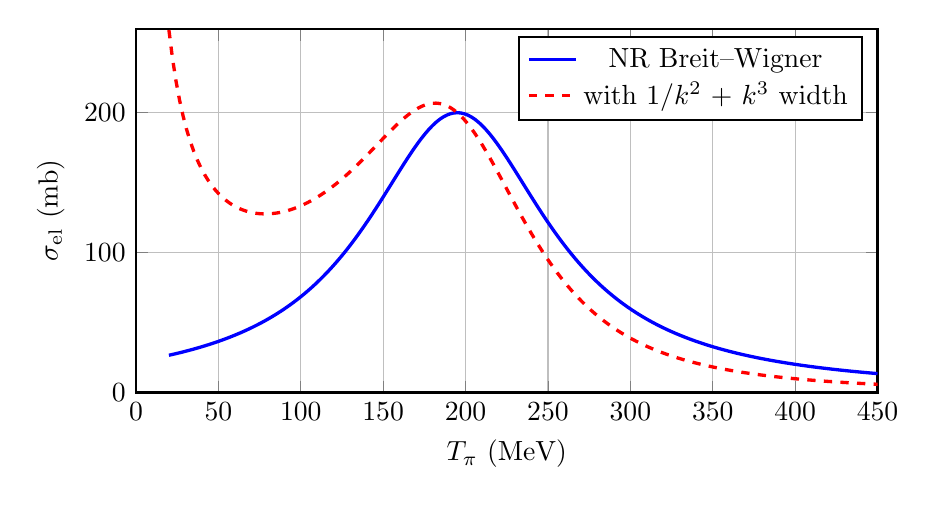
\begin{tikzpicture}
\begin{axis}[xlabel={$T_{\pi}$ (MeV)}, ylabel={$\sigma_\text{el}$ (mb)},
  xmin=0, xmax=450, ymin=0, ymax=260, width=11cm, height=6.2cm,
  samples=200, grid=both, thick]
\addplot[blue, very thick, domain=20:450] {200*((137/2)^2)/((x-195)^2+(137/2)^2)};
\addlegendentry{NR Breit--Wigner}
\addplot[red, dashed, very thick, domain=20:450] {200*((137/2)^2)/((x-195)^2+(137/2)^2)*((195/x))};
\addlegendentry{with $1/k^{2}$ + $k^{3}$ width}
\end{axis}
\end{tikzpicture}
\end{center}

\emph{Deviations from \eqref{eq:BW-NR}.}
\begin{enumerate}
\item Prefactor $1/k^{2}$ skews the peak towards lower energies.
\item Energy-dependent $P$-wave partial width: $\Delta(J^{P}=3/2^{+})\to\pi N$ has $L=1$, hence $\Gamma_{\pi N}(E)\propto k^{2L+1}=k^{3}$. Phase-space suppression at low $T_{\pi}$, broadening at high $T_{\pi}$.
\item Non-resonant $S$-wave background and (above $\sim 400\,\text{MeV}$) onset of inelastic channels and the next resonance ($N^{*}(1440)$).
\end{enumerate}
The asymmetric shape (steep rise, slow fall) is the signature of the $P_{33}$ ($I=3/2,J=3/2,L=1$) state.

%==========================================================
\section*{Question 3 --- Born approximation and the deuteron}

\textbf{Problem.} Define the Born scattering amplitude; evaluate it for a Gaussian potential $U(r)=U_{0}e^{-r^{2}/2\sigma^{2}}$; compute $\sigma_\text{tot}$; estimate intrinsic nucleon momentum at $\sigma\sim 1\,\text{fm}$, deuteron $U_{0}$ from $|E|=2.2\,\text{MeV}$, and mean free path of $10\,\text{MeV}$ neutrons in water.

\subsection*{(a) Born amplitude and validity}

Asymptotic wavefunction: incoming plane wave plus outgoing spherical wave,
\[
\psi(\vb r)\xrightarrow{r\to\infty}e^{i\vb k\cdot\vb r}+f(\theta,\phi)\,\frac{e^{ikr}}{r}.
\]
Iterating the Lippmann--Schwinger equation once with unperturbed plane waves:
\begin{equation}
f^\text{Born}(\theta,\phi)\;=\;-\frac{m}{2\pi\hbar^{2}}\int e^{-i\vb q\cdot\vb r}\,U(\vb r)\,\de^{3}\bm r,\qquad\vb q=\vb k'-\vb k.
\label{eq:fBorn-def}
\end{equation}
\emph{Validity.} Scattered wave small inside the potential range, $|U|\,a\ll\hbar v$ at high $k$, $|U|\ll\hbar^{2}/(ma^{2})$ at low $k$; fails near bound states or resonances. (Convention below: $U$ has units of energy, $f=-(m/2\pi\hbar^{2})\tilde U(\bm q)$.)

\subsection*{(b) Forward Born amplitude for a Gaussian}

Elastic: $|\vb k|=|\vb k'|=k$, momentum transfer
\[
q^{2}\;=\;|\vb k-\vb k'|^{2}\;=\;2k^{2}(1-\cos\theta).
\]
Fourier transform of the Gaussian (factorise into three 1D integrals):
\[
\tilde U(\bm q)\;=\;\int e^{-i\vb q\cdot\vb r}U_{0}e^{-r^{2}/2\sigma^{2}}\,\de^{3}\bm r\;=\;U_{0}(2\pi\sigma^{2})^{3/2}e^{-q^{2}\sigma^{2}/2}.
\]
Insert into \eqref{eq:fBorn-def}:
\[
f(\theta,k)\;=\;-\frac{m}{2\pi\hbar^{2}}\,U_{0}(2\pi\sigma^{2})^{3/2}\,e^{-q^{2}\sigma^{2}/2}.
\]
Substitute $q^{2}=2k^{2}(1-\cos\theta)$:
\[
f(\theta,k)\;=\;-\frac{m\,U_{0}(2\pi)^{3/2}\sigma^{3}}{2\pi\hbar^{2}}\,e^{-\sigma^{2}k^{2}(1-\cos\theta)}.
\]
Tidy the prefactor:
\begin{equation}
\boxed{\;f(\theta,k)\;=\;A\,e^{-\sigma^{2}k^{2}(1-\cos\theta)},\qquad A=-\frac{m\,U_{0}\,\sigma^{3}\sqrt{2\pi}}{\hbar^{2}}.\;}
\label{eq:Aresult}
\end{equation}

\subsection*{(c) Total cross-section}

Integrate $|f|^{2}$ over solid angle:
\[
\sigma_\text{tot}(k)\;=\;\int|f|^{2}\,\de\Omega\;=\;2\pi A^{2}\int_{0}^{\pi}e^{-2\sigma^{2}k^{2}(1-\cos\theta)}\sin\theta\,\de\theta.
\]
Substitute $u=1-\cos\theta$, $\de u=\sin\theta\,\de\theta$, $u\in[0,2]$:
\[
\sigma_\text{tot}(k)\;=\;2\pi A^{2}\int_{0}^{2}e^{-2\sigma^{2}k^{2}u}\,\de u.
\]
Evaluate the integral:
\[
\sigma_\text{tot}(k)\;=\;2\pi A^{2}\,\frac{1-e^{-4\sigma^{2}k^{2}}}{2\sigma^{2}k^{2}}.
\]
Tidy:
\begin{equation}
\boxed{\;\sigma_\text{tot}(k)\;=\;B\bigl(1-e^{-4\sigma^{2}k^{2}}\bigr),\qquad B=\frac{\pi A^{2}}{\sigma^{2}k^{2}}=\frac{2\pi^{2}m^{2}U_{0}^{2}\sigma^{4}}{\hbar^{4}k^{2}}.\;}
\label{eq:Bresult}
\end{equation}
Limits: $\sigma k\ll 1\Rightarrow\sigma_\text{tot}\to 4\pi A^{2}$ (constant, $S$-wave); $\sigma k\gg 1\Rightarrow\sigma_\text{tot}\to B\propto 1/k^{2}$.

\subsection*{(d) Intrinsic nucleon momentum at $\sigma\sim 1\,\text{fm}$}

Heisenberg, $\Delta r\sim\sigma$:
\[
p\;\sim\;\frac{\hbar}{\sigma}\;=\;\frac{197\,\text{MeV}\,\text{fm}}{1\,\text{fm}}.
\]
\begin{equation}
\boxed{\;p\;\sim\;200\,\text{MeV}/c.\;}
\end{equation}
Non-relativistic kinetic energy:
\[
T\;\sim\;\frac{p^{2}}{2m_{N}}\;=\;\frac{(200)^{2}}{2(940)}\,\text{MeV}\;\simeq\;21\,\text{MeV}.
\]

\subsection*{(e) Estimate of $U_{0}$ from $|E|=2.2\,\text{MeV}$}

Two-body deuteron: reduced mass $\mu=m_{p}m_{n}/(m_{p}+m_{n})\simeq m_{N}/2\simeq 470\,\text{MeV}/c^{2}$. Variational ansatz of width $\sigma$:
\[
E\;\approx\;\frac{\hbar^{2}}{2\mu\sigma^{2}}+U_{0}\,\langle e^{-r^{2}/2\sigma^{2}}\rangle.
\]
Take $\langle e^{-r^{2}/2\sigma^{2}}\rangle\sim 1$ for an order-of-magnitude estimate. Set $E=-2.2\,\text{MeV}$:
\[
\frac{(\hbar c)^{2}}{2\mu c^{2}\sigma^{2}}+U_{0}\;=\;-2.2\,\text{MeV}.
\]
Kinetic term:
\[
T\;=\;\frac{(197)^{2}}{2(470)(1)^{2}}\,\text{MeV}\;\simeq\;41\,\text{MeV}.
\]
Solve for $U_{0}$:
\[
U_{0}\;=\;-T-|E|\;=\;-41-2.2\,\text{MeV}.
\]
\begin{equation}
\boxed{\;U_{0}\;\simeq\;-43\,\text{MeV (attractive)}.\;}
\end{equation}
Canonical depth of the nucleon--nucleon well; binding is the small difference of two ${\sim}40\,\text{MeV}$ terms.

\subsection*{(f) Mean free path of a $10\,\text{MeV}$ neutron in water}

CM wavenumber for $E=10\,\text{MeV}$:
\[
\hbar c\,k\;=\;\sqrt{2m_{n}c^{2}\cdot E}\;=\;\sqrt{2(940)(10)}\,\text{MeV}\;=\;137\,\text{MeV}.
\]
Hence $k=137/197\,\text{fm}^{-1}=0.696\,\text{fm}^{-1}$, $\sigma k=0.696$, $4\sigma^{2}k^{2}=1.94$:
\[
1-e^{-4\sigma^{2}k^{2}}\;=\;1-e^{-1.94}\;=\;0.856.
\]
Compute $B$ from \eqref{eq:Bresult} using natural units. Group the prefactor:
\[
\frac{m_{n}c^{2}\,|U_{0}|\,\sigma^{2}}{(\hbar c)^{2}}\;=\;\frac{(940)(43)(1)^{2}}{(197)^{2}}.
\]
Evaluate:
\[
\frac{m_{n}c^{2}\,|U_{0}|\,\sigma^{2}}{(\hbar c)^{2}}\;=\;\frac{40\,420}{38\,809}\;=\;1.041.
\]
Hence
\[
B\;=\;\frac{2\pi^{2}}{(\sigma k)^{2}}\,(1.041)^{2}\,\sigma^{2}\;=\;\frac{2\pi^{2}(1.084)}{0.484}\,\text{fm}^{2}.
\]
Evaluate:
\[
B\;\simeq\;44.2\,\text{fm}^{2}\;=\;0.442\,\text{barn}.
\]
Total cross-section:
\[
\sigma_\text{tot}\;=\;B\times 0.856\;=\;0.378\,\text{barn}\;=\;3.78\times 10^{-25}\,\text{cm}^{2}.
\]

Hydrogen number density in water ($\rho=1\,\text{g/cm}^{3}$, $M=18\,\text{g/mol}$, two H per molecule):
\[
n_{H}\;=\;\frac{2N_{A}\rho}{M}\;=\;\frac{2(6.02\times 10^{23})}{18}\,\text{cm}^{-3}\;=\;6.69\times 10^{22}\,\text{cm}^{-3}.
\]
Mean free path:
\[
\lambda\;=\;\frac{1}{n_{H}\,\sigma_\text{tot}}\;=\;\frac{1}{(6.69\times 10^{22})(3.78\times 10^{-25})}\,\text{cm}.
\]
Evaluate:
\begin{equation}
\boxed{\;\lambda\;\simeq\;40\,\text{cm}.\;}
\end{equation}
Order-of-magnitude consistent with the moderation length in light water (Born underestimates by $\sim 2$--$3$ near a nearly-bound channel).

%==========================================================
\section*{Question 4 --- SEMF, fission and reactor neutrinos}

\textbf{Problem.} Discuss the binding-energy-per-nucleon curve and the SEMF; estimate $\Delta E$ in the canonical $^{235}$U fission; rate of $\bar\nu_{e}$ from $10\,\text{GW}_\text{th}$; detector mass at $200\,\text{km}$ for 10 IBD events/month; explain factor-of-two suppression.

\subsection*{(a) Binding-energy curve and the SEMF}

\begin{equation}
B(A,Z)\;=\;a_{V}A-a_{S}A^{2/3}-a_{C}\frac{Z(Z-1)}{A^{1/3}}-a_{A}\frac{(N-Z)^{2}}{A}+\delta(A,Z),
\label{eq:SEMF}
\end{equation}
with $a_{V}\!\simeq\!15.8$, $a_{S}\!\simeq\!17.8$, $a_{C}\!\simeq\!0.71$, $a_{A}\!\simeq\!23.7\,\text{MeV}$; $\delta=\pm a_{P}A^{-1/2}$, $a_{P}\simeq 12\,\text{MeV}$.

\emph{Volume $+a_{V}A$.} Saturation of the short-range (${\lesssim}2\,\text{fm}$) NN force: each nucleon binds only to neighbours, contribution $\propto A$.

\emph{Surface $-a_{S}A^{2/3}$.} Surface nucleons miss neighbours; surface area $\propto R^{2}\propto A^{2/3}$. Dominant for light nuclei, drives the rise of $B/A$ from $A=1$ to ${\sim}20$.

\emph{Coulomb $-a_{C}Z(Z-1)/A^{1/3}$.} Self-energy of $Z$ protons in radius $\propto A^{1/3}$. Drives the slow decline beyond $A\!\gtrsim\!60$ and fission instability of the heaviest nuclei.

\emph{Asymmetry $-a_{A}(N-Z)^{2}/A$.} Pauli exclusion penalty for $N\neq Z$; favours $N=Z$ light nuclei but is overcome by Coulomb in heavy nuclei (valley of stability bends to $N>Z$).

\emph{Pairing $\pm a_{P}A^{-1/2}$.} Like-pair coupling to $J=0$: $+$ ee, $-$ oo, 0 odd-$A$.

\emph{Validity.} Best for $A\gtrsim 20$ away from closed shells; misses magic-number ($N$ or $Z=2,8,20,28,50,82,126$) and deformation effects. Maximum at $A\simeq 56$ (Fe), $B/A\simeq 8.8\,\text{MeV}$: fusion of light, fission of heavy, both release energy.

\subsection*{(b) Energy released per fission}

\[
\Delta E\;\simeq\;B(^{92}\text{Kr})+B(^{141}\text{Ba})-B(^{235}\text{U}).
\]
Read $B/A$ from the curve:
\[
B(^{235}\text{U})\;\simeq\;235\times 7.6\,\text{MeV}\;=\;1786\,\text{MeV}.
\]
\[
B(^{92}\text{Kr})\;\simeq\;92\times 8.7\,\text{MeV}\;=\;800\,\text{MeV}.
\]
\[
B(^{141}\text{Ba})\;\simeq\;141\times 8.4\,\text{MeV}\;=\;1184\,\text{MeV}.
\]
Sum (free neutrons unbound):
\[
\Delta E\;=\;800+1184-1786\,\text{MeV}.
\]
\begin{equation}
\boxed{\;\Delta E\;\simeq\;200\,\text{MeV}\text{ per fission}.\;}
\end{equation}

\subsection*{(c) Anti-neutrino rate from a $10\,\text{GW}_\text{th}$ reactor}

Each fission $\Rightarrow$ two neutron-rich daughters $\Rightarrow$ ${\sim}3$ $\beta^{-}$ each $\Rightarrow$ $\bar n_{\nu}\simeq 6$ $\bar\nu_{e}$/fission. Fission rate:
\[
R_\text{fiss}\;=\;\frac{P_\text{th}}{\Delta E}\;=\;\frac{10^{10}\,\text{J/s}}{200\,\text{MeV}\times 1.602\times 10^{-13}\,\text{J/MeV}}.
\]
Evaluate:
\[
R_\text{fiss}\;\simeq\;3.12\times 10^{20}\,\text{s}^{-1}.
\]
Anti-neutrino rate:
\[
R_{\bar\nu}\;=\;\bar n_{\nu}\,R_\text{fiss}\;=\;6\times 3.12\times 10^{20}\,\text{s}^{-1}.
\]
\begin{equation}
\boxed{\;R_{\bar\nu}\;\simeq\;1.9\times 10^{21}\,\bar\nu_{e}/\text{s}.\;}
\end{equation}

\subsection*{(d) Detector mass at $200\,\text{km}$ for 10 events/month}

Isotropic flux at $D=200\,\text{km}=2\times 10^{7}\,\text{cm}$:
\[
\Phi\;=\;\frac{R_{\bar\nu}}{4\pi D^{2}}\;=\;\frac{1.9\times 10^{21}}{4\pi(2\times 10^{7})^{2}}\,\text{cm}^{-2}\,\text{s}^{-1}.
\]
Evaluate:
\[
\Phi\;=\;\frac{1.9\times 10^{21}}{5.03\times 10^{15}}\;=\;3.78\times 10^{5}\,\text{cm}^{-2}\,\text{s}^{-1}.
\]
Above-threshold fraction $10\%$:
\[
\Phi_\text{eff}\;=\;0.10\,\Phi\;=\;3.78\times 10^{4}\,\text{cm}^{-2}\,\text{s}^{-1}.
\]

Free-proton density per gram of $\text{C}_{20}\text{H}_{34}$ ($M=20(12)+34=274\,\text{g/mol}$):
\[
n_{p}\;=\;\frac{34\,N_{A}}{M}\;=\;\frac{34(6.02\times 10^{23})}{274}\,\text{g}^{-1}.
\]
Evaluate:
\[
n_{p}\;\simeq\;7.47\times 10^{22}\,\text{g}^{-1}.
\]
Event rate per gram:
\[
r\;=\;n_{p}\,\sigma_\text{IBD}\,\Phi_\text{eff}\;=\;(7.47\times 10^{22})(4\times 10^{-42})(3.78\times 10^{4})\,\text{s}^{-1}\,\text{g}^{-1}.
\]
Evaluate:
\[
r\;\simeq\;1.13\times 10^{-14}\,\text{s}^{-1}\,\text{g}^{-1}.
\]
Counts per gram per month ($t=2.59\times 10^{6}\,\text{s}$):
\[
N_{1}\;=\;r\,t\;=\;1.13\times 10^{-14}\times 2.59\times 10^{6}\;\simeq\;2.93\times 10^{-8}\,\text{events/g}.
\]
Required mass for 10 events:
\[
M_\text{det}\;=\;\frac{10}{N_{1}}\;=\;\frac{10}{2.93\times 10^{-8}}\,\text{g}\;\simeq\;3.4\times 10^{8}\,\text{g}.
\]
\begin{equation}
\boxed{\;M_\text{det}\;\simeq\;340\,\text{tonnes}\;(\sim\!\text{kT scale, KamLAND-class}).\;}
\end{equation}

\subsection*{(e) Missing assumption}

Above calculation assumes flavour conservation in propagation. \emph{Neutrino oscillations} convert $\bar\nu_{e}\to\bar\nu_{\mu,\tau}$ over $L=200\,\text{km}$; IBD is sensitive only to $\bar\nu_{e}$. Survival
\[
P_{ee}\;\simeq\;1-\tfrac{1}{2}\sin^{2}2\theta_{12}\;\simeq\;0.55,
\]
in the KamLAND averaged regime ($\Delta m_{21}^{2}L/4E\gtrsim 1$ for $E\sim$ few MeV at $L\sim 200\,\text{km}$). Multiplies the predicted rate by $\sim 0.5$.
\begin{equation}
\boxed{\;\text{Missing assumption: neutrino oscillations.}\;}
\end{equation}

\end{document}
